%------------------------------------------------------------------------
%Editar Diplomado
\hypertarget{cv:modificarTermino}{\section{Modificar Término de Glosario}} \label{sec:modificarTermino}

	Esta funcionalidad le permitirá modificar la información de un término de glosario previamente registrado con el fin de corregir o actualizar datos del mismo. 

		\subsection{Procedimiento}

			%Pasos de procedimiento
			\begin{enumerate}
	
			\item Oprima el botón \IUEditar{} de algún registro existente de la pantalla \ref{fig:GestionarGlosario} ''Gestionar Términos de Glosario''.
	
			\item Se mostrará la pantalla \ref{fig:modificarTermino} ''Modificar Términos de Glosario''.
			
			%Pantalla
			\begin{figure}[htbp!]
				\begin{center}
					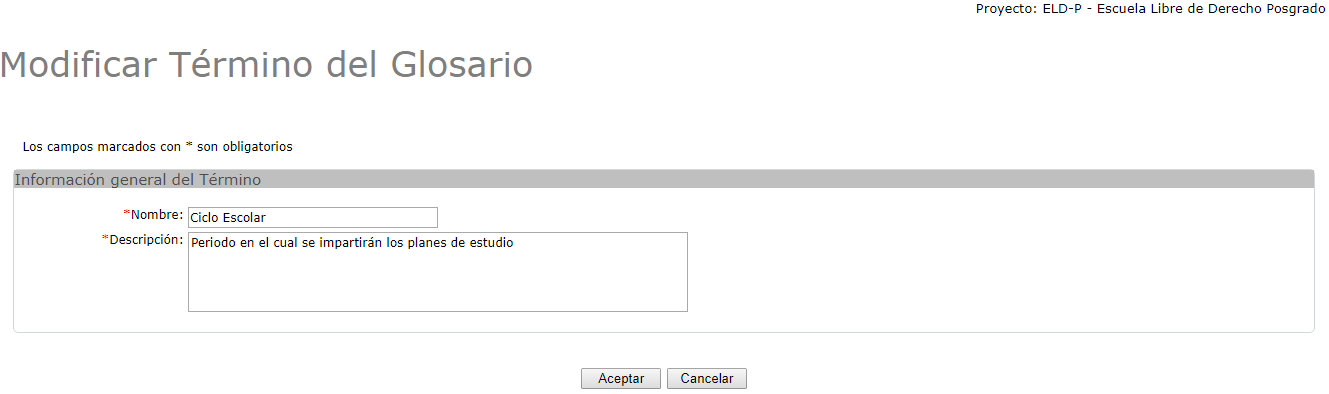
\includegraphics[scale=0.5]{roles/lider/glosario/pantallas/IU6-2modificarTermino}
					\caption{Modificar Término de Glosario}
					\label{fig:modificarTermino}
				\end{center}
			\end{figure}
		
			\item Modifique los datos solicitados por la pantalla.
						
			\item Oprima el botón \IUAceptar.
			
			\item Se mostrará el mensaje \ref{fig:terminoModificado} en la pantalla \ref{fig:GestionarGlosario} ''Gestionar Términos de Glosario''.
			
			\begin{figure}[htbp!]
				\begin{center}
					
\includegraphics[scale=0.5]{roles/lider/glosario/pantallas/IU6-2MSG1}
					\caption{MSG: Término Actualizado}
					\label{fig:terminoModificado}
				\end{center}
			\end{figure}
			\end{enumerate}